\documentclass[12pt,
openright, 
oneside,
%twoside, %TCC: Se seu texto tem mais de 100 páginas, descomente esta linha e comente a anterior
a4paper,
brazil]{facom-ufu-abntex2}

%\usepackage[disable]{todonotes}
\usepackage[colorinlistoftodos]{todonotes}	%use a linha anterior para esconder os todos.
\usepackage{amsthm}
\usepackage{listings}
\usepackage{forest}
\usepackage{listings}
\usepackage{xcolor}
\usepackage{minted}
\usepackage[portuguese, ruled, linesnumbered]{algorithm2e}

\definecolor{comment_green}{RGB}{0,128,0}

\lstset{
	language=C++,
    basicstyle=\ttfamily\tiny,
    stringstyle=\color{red},
    commentstyle=\color{comment_green},
    morecomment=[s][\color{blue}]{/**}{*/},
    extendedchars=true,
    showspaces=false,
    showstringspaces=false,
    numbers=left,
    numberstyle=\tiny,
    breaklines=true,
    breakautoindent=true,
    breakatwhitespace=true,
}
\newcommand{\codigo}{
}

\renewcommand{\lstlistingname}{Listagem}

\theoremstyle{definition}
\newtheorem{definition}{Definição}

\autor{José Augusto Bolina} %TCC
\data{2018}
\orientador{Lásaro Jonas Camargos} %TCC

\titulo{Revisitando o P4 Paxos} %TCC

\renewcommand{\thesection}{\arabic{chapter}.\arabic{section}}

\begin{document}

% ----------------------------------------------------------
% ELEMENTOS PRÉ-TEXTUAIS
% ----------------------------------------------------------
%\pretextual
\imprimircapa
\imprimirfolhaderosto

%\begin{resumo} %TCC:

% \vspace{\onelineskip}

% \noindent
% \textbf{Palavras-chave}: Acordo de Nível de Serviço (SLA), Monitoramento, Multicaminhos,
% OpenFlow, Qualidade de Serviço (QoS), Redes Definidas por Software. %TCC:

%\end{resumo}

%% ---
%% inserir lista de símbolos, se for adequado ao trabalho. %TCC:
%% ---


%\begin{siglas}
%\end{siglas}

%\begin{simbolos}
%  \item[$ \Gamma $] Letra grega Gama
%  \item[$ \Lambda $] Lambda
%  \item[$ \zeta $] Letra grega minúscula zeta
%  \item[$ \in $] Pertence
%\end{simbolos}
%% ---

% ---
% inserir o sumario
% ---
\pdfbookmark[0]{\contentsname}{toc}
\tableofcontents*
\cleardoublepage
% ---


% ----------------------------------------------------------
% ELEMENTOS TEXTUAIS
% ----------------------------------------------------------
\textual

% \todo{A estrutura do texto está excelente. A explicação do paxos está bem legal, mais detalhada do que esperava. É preciso falar mais na intro sobre o trabalho que estamos replicando (duas ou três linhas). Depois de terminar de preencher, precisaremos dar uma revisada no texto pois tem muitas redundâncias. Depois que tiver ficado um tempo sem ler, você mesmo as perceberá.}

% ######################### INICIO ###########################################
\chapter{Introdução}

Com o avanço da tecnologia a interação com a computação se tornou diária, mesmo
nos mínimos detalhes sempre se interage com algum software no dia a dia. Com
esse grande aumento na utilização de softwares e do aprimoramento de novas tecnologias, 
surge a necessidade de aplicações resilientes e tolerantes a falhas. 

Uma aplicação tolerante a falhas consegue manter o funcionamento mesmo com a eventual 
falha de um de seus componentes. Como é possível existir eventos inesperados que podem
causar a eventual falha - ou \textit{crash} - de um servidor, são necessários métodos
para garantir a consistência quando a aplicação retornar com seu funcionamento
normal. 

Uma maneira de possuir uma aplicação tolerante a falhas é a replicação de máquinas
de estado, onde o serviço é modelado como uma máquina de estados determinísticos, e o
serviço é executado em cada réplica \citep{santos2012state}, dessa maneira é mantida
a consistência da aplicação, mas um \textit{overhead} é adicionado na execução
de comandos, pois as réplicas precisam ser consistentes entre si. No centro da replicação
de máquina de estados, existe um problema de consenso, onde o conjunto de réplicas deve 
chegar a um consenso e decidir sobre qual é o estado válido e decidir sobre qual 
transição será realizada. 

Para alcançar o consenso e obter uma aplicação tolerante a falhas, o algoritmo
Paxos é extensivamente utilizado com esse intuito \citep{dang2016paxos}. 
O algoritmo realiza uma custosa trocas de mensagens entre seus agentes. Por se 
tratar de um ambiente distribuído as mensagens podem demorar um tempo arbitrário 
para chegar ao destinatário ou se perder durante a transmissão. Para conseguir 
uma melhora na performance na execução do algoritmo, pode-se realizar a 
implementação do Paxos no dispositivos físicos da rede \citep{dang2016paxos}.

Com a utilização da linguagem P4, é aberta a possibilidade de se programar dispositivos
de rede. Com a utilização de uma tabela \textit{match+action} é possível 
realizar um processamento customizado dos pacotes sendo transportados, de forma a
se diminuir a latência do algoritmo e os pacotes atravessariam menos \textit{hops}.

Alguns exemplos de aplicações que realizam replicação de máquinas de estados, são,
por exemplo OpenReplica \citep{openreplica} e Google Chubby \citep{27897}. Aplicações
de replicação são críticas em data centers, que precisam sempre manter o serviço 
disponível, com informações consistentes, logo, a maneira como um algoritmo de consenso
funciona para realizar a replicação de máquina de estados influencia na performance 
de um data center.

O presente trabalho se baseia no trabalho de Tu Dang et. al. \citep{dang2016paxos}, publicado
em 2016. Tal trabalho possui visões promissoras para o desenvolvimento
e pesquisa nas linguagens de programação de planos de dados e vislumbra o que pode ser
novos desafios nas pesquisas de protocolos de consenso. O presente projeto dá atenção maior
ao primeiro fator citado, realizando a implementação do algoritmo de consenso Paxos utilizando
a linguagem de programação de planos de dados P4.

\section{Justificativas}
Com a utilização do algoritmo Paxos para resolução do problema de consenso e para a 
construção de uma aplicação tolerante a falhas, é necessário uma comunicação entre os 
agentes pertencentes a aplicação. Essa comunicação, pode se tornar dispendiosa, pois 
a troca de mensagens entre as partes podem ter falhas e ser prolongada até que o 
algoritmo alcance seu objetivo que é o consenso.

Desta forma, essa comunicação poderiam influenciar na performance da aplicação e em 
sua disponibilidade, visto que esse processamento é realizado pela própria aplicação ou 
em servidores que tem essa função delegada. Visando esse problema, com a transferência
da lógica de consenso da aplicação para dispositivos de rede, podemos reduzir a latência
quando comparada a uma implementação em um servidor, e também é possível obter uma melhora
na taxa de transferência, visto que um algoritmo como o Paxos é um serviço que possui
alta comunicação entre as partes e não um algoritmo com alto processamento
\citep{netchainRtt}.

Desta maneira, o presente projeto busca obter uma melhora na performance de 
execução do Paxos e obter uma resposta do algoritmo de forma mais rápida e menos 
custosa, realizando a implementação do algoritmo em dispositivos de rede.

\section{Objetivos}
Com a possibilidade de programação em dispositivos de redes, o presente trabalho 
visa realizar a implementação do algoritmo Paxos nos dispositivos de rede, especificamente
\textit{switches}, utilizando a linguagem $P4_{14}$. 
Desta maneira, conseguindo uma melhora na performance do algoritmo, pois uma parte 
que seria executado em um servidor se moveria para ser executado nesses dispositivos, permitindo,
assim, processar as mensagens enquanto as mesmas estão sendo roteadas e atravessar menos
\textit{hops}, resultando na redução da latência.

Inicialmente, alcançando os resultados obtidos no projeto de Tu Dang et. al. 
\citep{dang2016paxos}, como citado pelos pesquisadores do projeto passado e, 
como um dos principais pontos deixado pelos pesquisadores seria em relação ao desenvolvimento
e evolução das linguagens de programação de plano de dados, um dos objetivos seria 
também uma nova perspectiva acerca das linguagens de programação de planos de dados, 
especificamente a linguagem P4.

\section{Método}
O método utilizado para o desenvolvimento do projeto foi divido em três partes, para
ser realizado uma análise em cada uma das partes do projeto separadamente, assim deixando uma
visão mais clara acerca do decorrer do projeto.

\subsection{Fase 1}
Replicação do projeto de Tu Dang et. al. \citep{dang2016paxos} utilizando a linguagem 
$P4_{14}$, realização de simulações para verificar o funcionamento do projeto.

\subsection{Fase 2}
Após realizada a replicação, será realizada uma verificação de possíveis fatores que podem ser 
melhorados no antigo projeto, onde será explicado o que pode ser feito para melhorar e como será
realizada a implementação.

\subsection{Fase 3}
A terceira e última fase será composta pela implementação e análise das melhorias, serão realizadas
simulações também utilizando o Mininet para verificação do comportamento na rede e uma comparação
entre a nova e atual versão do projeto e possíveis pontos para futuras aplicações e pesquisas.

\section{Cronograma}
O projeto será realizado em dois semestres, cada semestre compreende 18 semanas, sendo assim,
um tempo total de desenvolvimento de 36 semanas ou aproximadamente 8 meses. A tabela 
\ref{tab:atividades} demonstra como serão realizadas as atividades no decorrer dos meses. 
% \todo{preferiria um cronograma semana a semana, dado que o prazo de execução é tão curto}

\begin{table}[h!]
    \begin{tabular}{|p{8cm}|c|c|c|c|c|c|c|c|}
    \hline
    Atividades & 1 & 2 & 3 & 4 & 5 & 6 & 7 & 8 \\
    \hline
    \hline
     
    Revisão trabalhos correlatos & X & X & & & & & &  \\
    \hline 
    
    Revisão Paxos & & X & X & & & & & \\
    \hline
    
    Revisão P4 & & & X & X & & & & \\
    \hline
    
    Primeira fase do método & & & & X & & & & \\
    \hline
    
    Segunda fase do método & & & & & X & & & \\
    \hline
    
    Terceira fase do método & & & & & & X & & \\
    \hline
    
    Correção da monografia & & & & & & & X & \\
    \hline
    
    Monografia & & X & X & X & X & X & & \\
    \hline
    
    Defesa do trabalho de conclusão de curso & & & & & & & & X \\
    \hline
\end{tabular}
    \caption{Tabela de atividades}
    \label{tab:atividades}
\end{table}

%######################### FUNDAMENTACAO ##################################
\chapter{Fundamentação Teórica}
Esse capítulo manterá o foco em detalhar e explicar as técnicas utilizadas para realização 
do projeto. Não serão abordadas questões de implementação, serão explicadas somente de modo
teórico, a fim de auxiliar o entendimento do leitor.

\section{Referencial Teórico}
Para seguirmos uma linha de raciocínio linear, e melhorar entendimento da teoria
para compreender o projeto, será abordado inicialmente informações sobre o 
algoritmo Paxos, seu modo de operar e flexibilidade para resolução de problemas.

Em seguida, será explicado como é o funcionamento da linguagem P4, alguns exemplos
da sintaxe e como suas definições na versão $P4_{14} - 1.0.5$. para finalizar o 
referencial teórico, será  explicado sobre o Mininet, seu funcionamento e qual o 
intuito na sua utilização no projeto.

\subsection{Paxos}
Paxos foi criado por Leslie Lamport, foi publicado inicialmente em 1989. Ele consiste em uma 
família de algoritmos voltada para resolução de problemas de consenso. 

A ideia de consenso é a de compartilhar informações entre um grupo de elementos
processadores, de preferência com uma maneira tolerante a falhas \citep{barborak1993consensus}.
Normalmente esse compartilhamento de informações é realizado com o intuito de tomar
uma decisão, por exemplo, os elementos devem decidir se \textit{commitam} ou não
uma transação realizada no banco de dados. 

De maneira básica, os elementos devem propor valores para serem escolhidos, 
comunicar entre si para tomar uma decisão e o valor final é escolhido pela maioria de 
elementos do conjunto.
A escolha da maioria não é necessariamente $\frac{n}{2}+1$, --- sendo $n$ o número
total de elementos processadores --- a decisão do que será maioria para tomada de decisão
pode ser criada pelo projetista, mas sempre visando atender o projeto, levando
em consideração que dentre esses $n$ elementos existirão alguns que falharão, essa maioria
é o quorum.

Para garantir a escolha de um valor e a propagação do valor decidido, o problema
possui alguns requisitos que devem ser atendidos pelos algoritmos. Os requisitos de
segurança são:

\begin{itemize}
    \item Um valor proposto talvez seja aceito
    \item Os elementos não aprendem qual o valor decidido até que um valor 
    tenha sido realmente decidido
    \item Um único valor é decidido
\end{itemize}

Algoritmos para consenso funcionam em estágios que refletem o próprio problema, e para
serem algoritmos tolerante a falhas, devem estar preparados para repetir esses ciclos,
considerando os valores escolhidos no ciclo passado, cada um desses ciclos é conhecido como
\textit{round} \citep{camargos2008multicoordinated}.

Os elementos participantes do Paxos, chamados de agentes, comunicam entre si, e assumem 
um ou mais papéis para a evolução do algoritmo. Os papéis a serem desempenhados são, 
utilizando a nomenclatura fornecida por Lamport \citep{lamport2001paxos}, 
\textit{proposers} (agentes que propõem algum valor), \textit{acceptors} 
(agentes que escolhem um único valor) e \textit{learners} (agentes que aprendem
qual foi o valor escolhido pelo algoritmo).
Existem alguns papéis de coordenadores, que podem ou não ser utilizados no algoritmo, 
sendo, por exemplo \textit{distinguished proposer}, que será explicado mais ao fim.

A comunicação dos agentes se dá por troca de mensagens, utilizando um modelo assíncrono e
não-bizantino, onde os agentes operam em diferentes velocidades, podem falhar e podem ser
resetados. Os agentes possuem um espaço de memória não volátil para armazenar informações e
as mensagens podem levar um tempo arbitrário para serem entregues, podem ser perdidas e/ou 
duplicadas, mas nunca corrompidas \citep{lamport2001paxos}.

\subsubsection{Escolha do valor}
A explicação para o entendimento do Paxos será iniciada pela escolha de um valor. 
Quando uma mensagem, com algum valor proposto chega para o \textit{acceptor}, esse valor pode 
ser aceito ou não. Logo, um \textit{acceptor} deve ser capaz de aceitar um valor proposto, 
assim sendo, sua definição é dada por:

\begin{definition}
$P_1$: um \textit{acceptor} deve aceitar o primeiro valor que receber.
\end{definition}

Mas para se chegar a um consenso e um único valor ser decidido pelos agentes, cada um
dos agentes deve ter escolhido o mesmo valor. Desta forma, os \textit{acceptors} devem
ser capazes de aceitar mais de uma proposta e também devem conseguir identificar qual
a proposta aceita, onde cada \textit{acceptor} possui um histórico de quais foram as
propostas aceitas.

As propostas enviadas devem possuir um identificador, passível de ser ordenado e que não 
possa ser repetido por outra proposta de modo a impossibilitar diferentes propostas com o mesmo
identificador no algoritmo. Adiante, as propostas serão simbolizadas por 
\textit{(n, v)}, sendo $n$ a identificação da proposta e $v$ o valor da mesma.

Para que os \textit{acceptors} escolham mais de uma proposta, deve-se existir a garantia de
que todas as propostas enviadas possuam o mesmo valor. Disso, surge a seguinte definição:

\begin{definition}
$P_2$: se uma proposta $(n, v)$ foi decidida, então todas propostas escolhidas com 
identificador $>n$ devem possuir valor $v$.
\end{definition}

Como os identificadores podem ser ordenados, a propriedade de que somente um valor é escolhido
é mantida pelo algoritmo. Como, para ser decidida, uma proposta tem que ter sido escolhida
por pelo menos um \textit{acceptor}, para fortalecer $P_2$, surge a seguinte definição:

\begin{definition}
$P_2^a$: se uma proposta $(n, v)$ foi decidida, então todas propostas com identificador
$>n$ escolhidas por um \textit{acceptor}, possui valor $v$.
\end{definition}

Como ainda existem cenários onde a definição de $P_2$ pode ser violada, a mesma precisa ser
reforçada. Um desses cenários, exemplificado por Lamport, é o seguinte:
Sempre se mantem $P_1$ para uma proposta ser escolhida, mas como
a comunicação é assíncrona, uma proposta pode ser escolhida por um \textit{acceptor c} 
que nunca tenha escolhido nenhuma proposta antes, e como os agentes podem falhar, suponha
que um \textit{proposer} envie uma proposta com identificador maior e com um valor qualquer.
O \textit{acceptor c} escolheria essa proposta, o que violaria a definição $P_2^a$. Para
fortalecer a definição, se tem o seguinte:

\begin{definition}
$P_2^b$: se uma proposta $(n, v)$ foi decidida, então todas propostas com identificador
$>n$ enviadas por um \textit{proposer}, possui valor $v$.
\end{definition}

Finalmente, para assegurar $P_2$, se tem a seguinte definição:

\begin{definition}
$P_2^c$: Para qualquer proposta $(n, v)$ enviada, existe um conjunto $S$ de
\textit{acceptors}, que cairá em um dos casos:

\begin{enumerate}
    \item $S$ não possui nenhum \textit{acceptor} que tenha escolhido uma proposta com 
identificador $<n$.

    \item $v$ é o valor da proposta com o maior identificador dentre as propostas com o 
menor identificador $<n$ escolhidas pelo conjunto $S$.
\end{enumerate}
\end{definition}

Com essas definições, o algoritmo para envio de propostas funcionará da seguinte maneira:

\begin{itemize}
    \item[]\textit{Proposer} envia proposta com identificador $n$ para conjunto de 
\textit{acceptors}, esperando uma das seguintes respostas:

    \begin{itemize}
        \item[] Promessa de não aceitar valor $<n$
        \item[] Se existir, proposta com maior identificador $<n$
    \end{itemize}
    
    \item[]Se receber uma resposta da maioria dos \textit{acceptors}:
    \begin{itemize}
        \item[] Enviar a proposta $(n, v)$, sendo $v$ o valor da proposta de maior identificador
        recebido nas respostas
        \item[] Um valor escolhido pelo próprio \textit{proposer}.
    \end{itemize}
\end{itemize}

Esses passos do algoritmo receberam um nomenclatura, que são \textit{prepare} e
\textit{accept}, respectivamente. O algoritmo em pseudo-código fica da seguinte maneira:

\begin{algorithm}[H]
\caption{Envio de propostas}
\SetAlgoLined
\Inicio{
$A$ = conjunto de \textit{acceptors}

$n$ = identificador

$respostas$ = []

\Para{cada $a \in A$}{
    $resposta$ = prepare($n$)
    
    adicione $resposta$ em $respostas$
}

\Se {aceito pela maioria}{
        $v$ = $v$ da proposta com maior identificador $\in respostas$ ou algum valor proposto
        
        \Para{cada $a \in A$}{
            accept($(n, v)$)
        }
    }
}
\end{algorithm}

Com esse algoritmo para envio de propostas, tem-se que um \textit{acceptor} irá
receber requisições do tipo \textit{prepare} e \textit{accept}. Para evitar um \textit{overhead}
de requisições e mensagens, o \textit{acceptor} pode ignorar requisições de qualquer tipo,
mas pode responder requisições do tipo \textit{prepare} se, e somente se, não estiver
prometido a outra proposta. Assim, para finalizar, tem-se:

\begin{definition}
$P_1^a$: um \textit{acceptor} pode aceitar qualquer proposta $(n, v)$, se, e somente se, não tiver
respondido um requisição \textit{prepare} com identificador $>n$.
\end{definition}

Desta forma, o algoritmo para envio de proposta está totalmente definido. Para se definir
o algoritmo para escolha de valores, deve-se assegurar que um \textit{acceptor} se
lembre da proposta com maior identificador que já escolheu e do maior identificador
que a requisição de \textit{prepare} respondeu. Essas informações devem ser mantidas
em uma memória não volátil, para que não sejam perdidas em eventuais falhas.

O algoritmo final para escolha é definido a seguir, separado em duas fases:

\begin{itemize}
    \item [Fase 1]
    \begin{itemize}
        \item [a] Um \textit{proposer} envia um requisição de \textit{prepare} com
        identificador $n$.
        
        \item [b] Se um \textit{acceptor} recebe um \textit{prepare} com identificador
        $n$ sendo o maior identificador que já recebeu, responde com a promessa de não
        aceitar nenhuma proposta com identificador $<n$, juntamente com a proposta com
        maior identificador $<n$, se existir.
    \end{itemize}
    
    \item [Fase 2]
    \begin{itemize}
        \item [a] Se o \textit{proposer} recebe resposta de uma maioria de \textit{acceptors}
        para seu \textit{prepare} de identificador $n$, então, envia um \textit{accept} 
        com identificador $n$ e valor $v$, sendo $v$ o valor da resposta de \textit{prepare}
        com maior identificador; senão, $v$ é um valor escolhido pelo \textit{proposer}.
        
        \item [b] Se um \textit{acceptor} recebe um \textit{accept} com identificador $n$,
        ele o aceita; caso, no tempo transcorrido tenha respondido um \textit{prepare}
        com identificador $>n$, poderá negar o \textit{accept} recebido.
    \end{itemize}
\end{itemize}

Após o valor ser decidido pelo algoritmo, o valor deve ser propagado para os \textit{learners},
que só conhecem o valor após ser definitivamente decidido.

\subsubsection{Propagação do valor decidido}
Após um valor ser decidido, os \textit{learners} devem conhecer o valor. Isso pode ser realizado
de diferentes maneiras e fica a critério do arquiteto para escolher qual atende melhor o
problema a ser resolvido.

Uma das maneiras de se conhecer o valor, seria cada um dos \textit{acceptors} responder para
todos os \textit{learners} qual o valor decidido. Assim, uma troca de $(n \cdot m)$ mensagens, 
o produto entre o número de \textit{acceptors} e o número de \textit{learners}, seriam obtidas.

Levando em consideração o papel de coordernador, citado anteriormente outra maneira de se 
realizar a propagação de mensagens seria os \textit{acceptors} enviarem o valor decidido para um
\textit{distinguished learner} que, após conhecer o valor decidido, envia para os
\textit{learners} tal valor decidido. Esse método teria $(n + m)$ troca de mensagens,
a soma entre o número de \textit{acceptors} e o número de \textit{learners}. Mas, como os
agentes são suscetíveis a falhas, o \textit{distinguished learner} também pode falhar,
assim impossibilitando a transmissão do valor decidido para os \textit{learners}.

\subsection{P4}
P4 é uma linguagem utilizada para programação do plano de dados em  dispositivos de 
rede \citep{paxos16spec}. Dispositivos de rede possuem dois planos, sendo eles o 
plano de controle e o plano de encaminhamento, também chamado de plano de dados ou 
plano do usuário. 

Pode ser feita uma analogia para se entender a diferença entre o 
plano de controle e o plano de dados, foi eleito de forma honesta, um novo 
funcionário para cuidar do transporte público da cidade Zanzizânia. Antes de se 
enviar os veículos é necessário realizar o planejamento de quais o caminhos serão
utilizados, as pessoas ainda não foram movidas pelos veículos, mas os caminhos 
e as paradas são conhecidos, essa parte é semelhante ao plano de controle, onde 
são encontradas as rotas.\citep{dataVsControl}.

Numa rede de roteadores, esse planejamento, que é descobrir e aprender novas rotas 
pode ser realizado por rotas estáticas, onde o roteador é ensinado sobre redes remotas
e como acessar essas redes. Pode também ser utilizado protocolos de roteamento dinâmicos,
onde os roteadores aprendem entre si sobre a existência de redes remotas.\citep{dataVsControl}.

Com o plano de rotas definidos para a cidade, agora é possível transportar os cidadãos
para os locais desejados através das ruas. Isso se trata do plano de dados, onde 
um pacote chega e é transportado para outro local, ou interface, através das rotas 
conhecidas \citep{dataVsControl}.

A linguagem P4 trabalha exatamente com o objetivo de expressar como os pacotes serão 
processados pelo plano de dados em um dispositivo de redirecionamento programável, 
como placas de redes, FPGA, switch em software, e ASICs \citep{paxos16spec}. Existe 
protocolo de comunicação como o OpenFlow, em que é possível controlar o fluxo dos 
pacotes de um roteador ou switch, mas para isso, é necessário explicitar os 
cabeçalhos em que se está trabalhando, tal método causou um aumento na complexidade 
especificação da linguagem enquanto não a tornou flexível para se adicionar campos 
nos cabeçalhos \citep{bosshart2014p4}.

Com isso, a P4 veio para ser independente do protocolo com que se está trabalhando,
vide seu nome no artigo em que foi publicado, 
\textit{Programming protocol-independent packet processor}. A linguagem foi 
construída visando a reconfigurabilidade e ser independente do dispositivo em que se 
deseja trabalhar, ou seja, é possível processar e analisar os pacotes enquanto o programador
não precisa se preocupar com detalhes do switch, onde esse trabalho fica para o compilador 
em transformar um código independente em um código para o dispositivo em que se vai 
trabalhar \citep{bosshart2014p4}.

\subsubsection{Funcionamento da linguagem}

A máquina abstrata que representa o funcionamento da linguagem é o de um dispositivo
de alto desempenho para o processamento de pacotes, esse modelo é chamado de PISA,
um acrônimo $Protocol-Independent Switch Architecture$, que possui alguns componentes
básicos, esses componentes também são definidos pela linguagem. O primeiro desses 
componentes é o parser programável, podendo ser definido pelo programador, juntamente 
com seu funcionamento. O segundo componente, o coração do modelo, é um pipeline de tabelas,
que combinam com algum dado e executam a ação correspondente. Após o pipeline, e executado
o processamento, o pacote passa por um $deparser$, que faz a função "inversa" do parser,
preparando o pacote na forma correta para ser transmitido \citep{p4LangTutorial}.

\begin{figure}[h]
    \caption{Protocol Independent Switch Architecture}
    \centering
    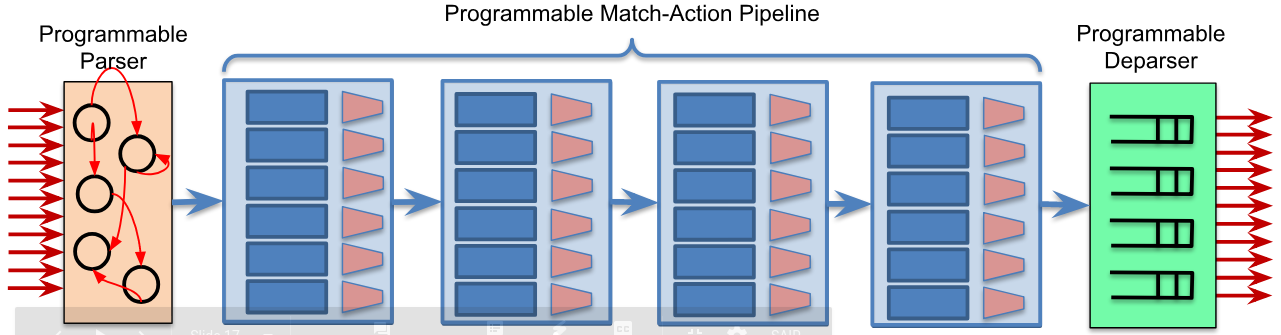
\includegraphics[width=\textwidth]{images/pisa.png}
    \label{fig:pisa-model}
\end{figure}

De forma geral, a linguagem funciona de forma bem direta, onde o programador define
os cabeçalhos que serão utilizados, assim, quando um novo pacote chega para processamento
seus campos são separados em campos individuais de acordo com as regras descritas e são
passados para as tabelas. As tabelas possuem como entrada os campos do cabeçalhos e 
resultados parciais, com essas informações, as tabelas executam diferentes ações,
como remover ou adicionar cabeçalhos, funções aritméticas e mover valores. Após o 
processamento pelas tabelas, as informações são passadas para o deparser, que 
monta os pacotes e transmite de volta para rede \citep{p4LangTutorial}.

\subsubsection{Componentes da linguagem}

A linguagem utiliza um modelo abstrato para redirecionamento de pacotes, que possui
dois tipos de operações, \textit{configure} e \textit{populate}. Durante a operação
de \textit{configure}, o parser é criado, é definida a ordem de estágios nas tabelas
\textit{match+action} e quais os campos do cabeçalhos são processados em cada estágio,
durante a operação de \textit{populate} adicionam e removem entradas nas tabelas
\textit{match+action} construídas durante operação de \textit{configure}. Assim,
durante \textit{configure}, é definido qual protocolo será utilizado e como será
o processamento dos pacotes, e durante \textit{populate} é determinada qual a 
política utilizada nos pacotes \citep{bosshart2014p4}.

A linguagem possui alguns componentes centrais, o primeiro desses componentes 
é o cabeçalho, cada cabeçalho é definido seguindo o nome do campo em conjunto 
com seu tamanho, campos que possui tamanho variável, devem ser definidos com o
tamanho máximo que esse campo pode possuir, um exemplo da definição de cabeçalho
seria:

\lstinputlisting[language=c++, caption={header.p4}]{code/p4-example/header.p4}

Outro componente é o parser, o parser especifica quais campos do cabeçalhos estão
bem definidos e como encontrar esses campos. Os campos extraídos dos cabeçalhos e 
são enviados para tabela de \textit{match+action}, onde será processado e seguirá
para o próximo passo, agindo de maneira semelhante a uma máquina de estados, em 
que as transições são realizadas por valores nos campos do cabeçalho. Um parser
segue a seguinte definição:

\lstinputlisting[language=c++, caption={header.p4}]{code/p4-example/parser.p4}

O parser é iniciado em \texttt{start}, é segue até encontrar um \texttt{stop} ou não
encontrar nenhum match, o que seria um erro \citep{bosshart2014p4}. O parser cria um 
\textit{parsed packet} em que a tabela de \textit{match+action} irá utilizar,
assim, valores que serão utilizados no processamento devem estar contidos nesse
\textit{parsed packet} \citep{p4USITutorial}.

O componente fornecido pela linguagem para o processamento dos pacotes são as tabelas,
de acordo com matches em campos do cabeçalho, esse match  pode ser exato, parcial 
ou ser algum "coringa", são especificados quais as ações serão executadas no
pacote. Utilizando a definição da tabela, o compilador pode decidir quanta memória 
é necessária e qual o tipo de memória necessária \citep{bosshart2014p4}. A
tabela é um componente que aponta qual ação deve ser realizada, assim, não é a 
tabela que executa a ação em si. A definição da tabela segue a seguinte forma:

\lstinputlisting[language=c++, caption={header.p4}]{code/p4-example/table.p4}

Pela definição da tabela pode se notar assim, que a ação é outro componente presente
na linguagem. Com a ação, é possível criar comandos mais complexos para primitivas
presentes no cabeçalho dos pacotes \citep{bosshart2014p4}. Ações funcionam de
maneira imperativa através de suas primitivas, podendo modificar, adicionar ou 
remover campos do cabeçalho, alterar campos dos metadados, realizar operações
que mantém um estado \citep{p4USITutorial}. O exemplo da estrutura de uma ação
é a seguinte:

\lstinputlisting[language=c++, caption={header.p4}]{code/p4-example/action.p4}

Caso uma ação necessite de parâmetros para ser executada, como no exemplo com
\texttt{value} e \texttt{egr\_spec}, esses parâmetros são fornecidos pela tabela em tempo 
de execução \citep{bosshart2014p4}.

O último componente é o controle de programa, utilizando funções, condições e referências
a tabelas, é definido o fluxo de uma tabela para a próxima, assim, o controle de programa
consiste em um programa imperativo que descreve o fluxo entre tabelas \textit{match+action} 
\citep{bosshart2014p4}. Um exemplo de como é o controle do programa: 

\lstinputlisting[language=c++, caption={header.p4}]{code/p4-example/program.p4}

Para a implantação do programa definido em dispositivos de rede, é necessário realizar
a compilação para mapear a descrição que está independente para o alvo em que se deseja
trabalhar. A compilação do controle de programa é realizada em duas etapas, inicialmente
é gerada uma representação intermediaria, onde o programa é representado como grafo de
dependências entre tabelas, que é analisado para verificar dependências entre as tabelas
e verificar quais campos de cabeçalho podem ser processados em paralelo. A segunda etapa
utiliza o grafo resultante da primeira etapa, que é mapeado para utilizar os recursos
específicos do dispositivo alvo em que se vai trabalhar \citep{bosshart2014p4}.

\subsubsection{Ferramentas oferecidas}
Outras ferramentas também são oferecidas pelo P4 Lang Consortium, dentre elas estão o 
$behavioral model$, também chamado de $bmv2$ e o $p4c-bm$. O $behavioral model$ é utilizado 
para executar os programas escritos em P4, oferece também na linha de comando uma interface 
para popular as tabelas inicialmente, se conectando através de um servidor $thrift$ e podendo 
assim, por exemplo, definir qual a ação padrão de uma tabela. Através da linha de comando do 
$behavioral model$ também é possível configurar como será o $multicast$. Para executar esses 
comandos, é preciso fornecer a representação do programa P4 em formato $JSON$
\footnote{JavaScript Object Notation}, isso pode ser obtido utilizando o $p4c-bm$, que gera a 
representação pronta para ser utilizada no $behavioral model$.

Com a arquitetura e ferramentas definidas, é possível, por exemplo, implementar o roteamento 
de pacotes IPv4. Assim, é possível notar que para implementação do projeto, a utilização da P4
é uma ótima escolha, visto que ela é flexível para criação dos pacotes e campos de cabeçalho
para execução do Paxos, e é possível realizar uma implementação que não fique atada a 
dispositivos de rede específicos.

\subsection{Mininet}
Mininet é um simulador de redes, que executa uma coleção de hosts finais, switches, 
roteadores e links, em uma única máquina. Os programas que utilizam dessa rede, podem enviar
pacotes e estes são processados, de maneira semelhante a rede Ethernet \citep{mininetDocs}.
Desta forma, para o presente projeto, é possível construir a rede utilizando o Mininet, e 
assim ser testada a implementação do Paxos nos dispositivos dessa rede.

Internamente, o Mininet realiza a virtualização encontradas no kernel do Linux, onde é possível
iniciar e escalar mais rápido do que sistemas que emulam a rede utilizando máquinas virtuais
\citep{mininetDocs}. Nesse modelo de virtualização, um único sistema é separado em diversas
partes menores, cada um destes possuindo uma parcela do poder de processamento e links virtuais
\citep{mininetDocs}.

Com a instalação do Mininet, é possível definir topologias de forma rápida e prática, a partir
de um interface pela linha de comando ou utilizando uma API em Python para orquestração da rede.
A partir da linha de comando, é possível executar comandos em nós específicos da rede 
\citep{mininetDocs}. 

\subsubsection{CLI}
Para iniciar a interface do Mininet pela linha de comando, com a topologia
\textit{minimal}, que consiste em 2 processos hosts, 1 processo switch e 1 controlador
básico, basta executar \citep{mininetOrg}:

\begin{minted}{bash}
  $ sudo mn
\end{minted}

Outras opções de topologia podem ser passadas com o argumento \texttt{--topo}. Para se testar a
conectividade entre os hosts, basta executar:

\begin{minted}{bash}
  mininet> h1 ping -c 1 h2
\end{minted}

Para $h1$ descobrir o endereço de $h2$, ele realiza um ARP, fazendo com que o evento de 
\texttt{packet\_in} vá para o controlador. O controlador realiza um broadcast em todas as portas
com a mensagem de \texttt{packet\_out} no switch. Assim, quando $h2$ recebe a requisição ARP ele
envia uma resposta, que passa pelo controlador e retorna para $h1$, que agora conhece o endereço
de $h2$. Com $h1$ agora possuindo o endereço de $h2$, envia o \textit{echo request} utilizando
protocolo ICMP, e $h2$ responde com \textit{echo reply}.

\subsubsection{Python}
Utilizando a API em Python, também é possível definir diferentes topologias para a rede. Um
exemplo simples consiste em uma topologia que possui 2 hosts e 2 switches, distribuídos como
a figura \ref{fig:custom-topology-example}. Para se definir essa topologia, utilizando
Python, fica da seguinte maneira:

\lstinputlisting[language=python,
caption={custom-topology.py}]{code/ninet-example/topo-2sw-2host.py}

Iniciando o Mininet no terminal, indicando qual a topologia utilizada, com o seguinte comando:

\begin{minted}{bash}
  $ sudo mn --custom custom-topology.py --topo custom_topo
\end{minted}

A API em Python possuem três níveis, definidos como API em baixo nível, API em nível médio e API
em alto nível, essa distinção é feita com o intuito de se construir componentes de alto nível
a partir de componentes de baixo nível \citep{mininetDocs}.

Baixo nível consiste de classes para os nós e os links, utilizando instâncias dessas 
classes é possível construir uma rede. Essas classes são \texttt{Host}, \texttt{Switch} e
\texttt{Link} e suas subclasses \citep{mininetDocs}.

O nível médio da API, consiste da classe \texttt{Mininet}, que se trata de um container,
que encapsula a criação de nós e links da rede, assim como a sua configuração \citep{mininetDocs}.

Em alto nível consiste a abstração \texttt{Topo}, para que se possa criar modelos de topologias 
parametrizadas e reutilizáveis, de modo que esses modelos possam ser passados para Mininet
pela linha de comando.

\begin{figure}[h]
    \caption{Topologia personalizada utilizando Python}
    \centering
    
\includegraphics[width=\textwidth]{images/2sw-2host.png}
    \label{fig:custom-topology-example}
\end{figure}

Visto que a utilização de verdadeiros switches e roteadores pode ser caro para simulação do
projeto, podemos utilizar a simulação que o Mininet oferece para resolver esse problema.
Como observado no exemplos, podemos utilizar diferentes topologias, que são criadas e 
executadas de forma prática, assim facilitando nos experimentos.

\section{Trabalhos Correlatos}
Essa seção visa listar trabalhos relacionados com o presente projeto, alguns destes usados
como material de referência para o desenvolvimento, esses trabalhos possuem experimentos
realizados previamente, utilizando ferramentas semelhantes as utilizadas no presente projeto 
e tais trabalhos deixaram áreas para futuras pesquisas sobre o tema.

\subsection{Paxos Made Switch-y}
Trabalho publicado em 2016, realizado por pesquisadores da Università della Svizzera italiana
e Université catholique de Louvain. Neste trabalho, foi realizada uma pesquisa com o intuito
de se realizar a implementação do Paxos para dispositivos de rede utilizando a linguagem
de programação de plano de dados P4, onde os testes para isso foram utilizando o Mininet. 
A pesquisa realiza também uma discussão sobre as linguagens de programação de plano de dados,
em específico a linguagem P4, onde foi relatado que a implementação é uma
implementação não trivial para linguagem, também abordam pontos como tratamento de erros,
dentre outros pontos. Foi realizada também uma discussão sobre protocolos de consenso,
onde os protocolos normalmente só assumem uma conexão ponto-a-ponto, seria interessante a
construção de protocolos que assumem outras propriedades da rede, pois existe um avanço
no hardware utilizado, assim, a performance dos protocolos poderiam ser melhoradas 
\citep{dang2016paxos}.

%######################### DESENVOLVIMENTO ##################################
\chapter{Desenvolvimento}
O desenvolvimento do projeto seguirá como descrito no cronograma, sendo divido em 
3 fases. Para cada uma das fases realizadas, seguirá uma explicação do que foi realizado,
dos códigos utilizados e uma breve explicação de qual o intuito que se deseja realizar.

O desenvolvimento foi realizado em uma máquina 64 bits utilizando Linux, especificamente a 
distribuição $Arch$ com o $kernel 4.20.1-arch1-1-ARCH$, possuindo processador Intel i3-3217U
que possui 4 núcleos, sendo 2 físicos e 2 virtuais com $clock$ 1.8 GHz e com 11454 MB de 
memória RAM.

\subsection{Fase 1}
Nessa subseção descreverá como se deu a replicação do projeto de Tu Dang et. al. 
\citep{dang2016paxos}, como foi realizada a criação do ambiente e quais foram os testes
realizados. O código utilizado no projeto passado pode ser encontrado no $GitHub$
\footnote{https://github.com/usi-systems/p4xos-public}, possuindo os passos que
se deve realizar para execução do projeto e dos testes. Para o presente projeto foi 
criado um repositório contendo todo código, que também pode ser encontrado no $GitHub$
\footnote{https://github.com/jabolina/monography-code}, desta forma ficando aberto
para contribuições e para ser utilizado em outras pesquisas e projetos.

\subsubsection{Ambiente}
Para execução do projeto, é criada uma máquina virtual que utiliza $Vagrant$ para
manutenção, instalação das dependências e pacotes necessários. O sistema operacional
utilizado é o Ubuntu, da imagem $ubuntu/trusty64$, fornecido pela própria
$Vagrant$ \citep{ubuntuTrusty}. Para o funcionamento é necessário indicar qual será
o provedor, para o projeto foi utilizado como provedor a $VirtualBox$, onde foi
alocado 2048 $MBs$ de memória RAM e 2 núcleos do processador para a máquina
virtual.

As dependências instaladas são descritas no arquivo $Vagrantfile$, nesse caso,
as dependências são descritas em scripts $bash$, que funcionam como forma
de provisão para máquina, podendo ser scripts que simples que criam pastas e arquivos
como também para instalação e preparação do ambiente, como é o caso. O primeiro script 
instala o Mininet, utilizando a versão que possui a $tag 2.2.1$, logo após é instalado 
o $POX$, que se trata de um $framework$ para comunicação com os $switches$ podendo 
utilizar tanto o protocolo $OpenFlow$  como $OVSDB$ \citep{poxWiki}. Para o $POX$ 
é utilizado um $commit$ específico. Um segundo script irá instalar as dependências 
relacionadas a P4, a primeira dependência é o $thrift$ que é utilizado por
algumas bibliotecas da P4. Em seguida são instalados dos repositórios da própria P4
as dependências $bmv2$ e $p4c-bm$, que são relacionadas a maneira de executar programas em P4.
Os programas em P4 são descritos em $JSON$ utilizando $p4c-bm$, depois as estruturas são 
carregadas no $bmv2$ utilizando a definição do arquivo $JSON$, assim é possível obter o modo
de roteamento desejado. Juntamente com as dependências, é clonado o repositório do projeto, 
com todo código necessário para executar testes.

\subsubsection{Teste}

Logando dentro da máquina virtual que se montou, é encontrado a implementação do projeto
passado, possuindo uma demonstração para utilização. Com essa demonstração, é possível
inserir valores relacionados a uma chaves e buscar por valores dado uma chave, utilizando
a linha de comando do Mininet é possível simular falhas na rede. Existe também um $script$
para testar inserção e pesquisa de valores, o $script$ insere um valor, pesquisa pela chave
associada a esse valor e pesquisa por uma chave não existente.

\begin{figure}[h]
    \caption{Topologia da demonstração}
    \centering
    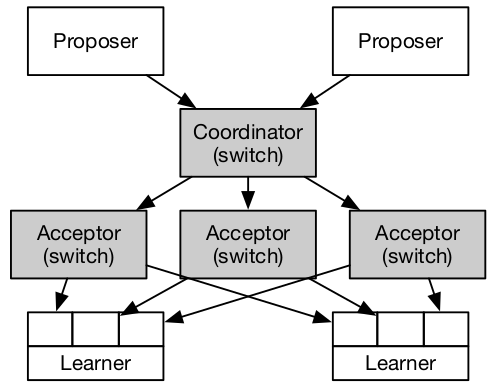
\includegraphics[scale=0.8]{images/arq.png}
    \label{fig:demo-topo}
\end{figure}

Essa demonstração e o projeto segue a topologia descrita por \ref{fig:demo-topo}, em que os
que estão coloridos em branco são executados em servidores.

\subsubsection{Funcionamento do projeto}
Para iniciar a execução da demonstração, é executado um script em Python, que irá definir a
topologia com o Minininet, que irá utilizar $switches$ programados, que executam os $acceptors$
e $coordinator$, com a topologia definida, as tabelas nos $switches$ são populadas, definindo
quais os valores utilizados na tabelas para executar o $match$ no tipo de mensagem, definindo o
grupo de $multicast$. Após execução do script, será possível realizar requisições no servidor
que foi aberto no $proposer$.

Quando o servidor recebe uma requisição, irá criar um novo pacote e inserir as informações no
cabeçalho para serem transportados, o formato do cabeçalho segue como definido em \ref{cod:p4-header}, 
possuindo o campo definindo o tipo da mensagem, com tamanho de 8 bits, o número da instância com tamanho 16 bits,
um campo definindo o round da instancia e o round em que o voto foi realizado, ambos com tamanho de
8 bits, o campo \texttt{acceptor} contém o identificador do $switch$ com tamanho de 64 bits e o valor do
voto com tamanho de 512 bits.

\lstinputlisting[language=c,caption={Cabeçalho do P4xos}, label={cod:p4-header}]{code/p4xos/explanation/headers.p4}

Assim, o $propopser$ irá enviar a requisição, que irá chegar no $coordinator$. O $coordinator$ garante que
somente um processo envie uma mensagem para o protocolo para uma dada instância, isso garante 
que o protocolo irá finalizar e impõe uma ordenação nas mensagens, como existe somente um
$coordinator$ para identificação e ordenação das mensagens, uma simples sequência crescente pode ser
utilizada. A ação que o $coordinator$ deve executar, quando em posse de uma pacote válido do Paxos,
deve ser de definir o tipo de mensagem do protocolo, definir o valor do \texttt{round} como 0, pois
uma nova instância foi iniciada, ler da memória não-volátil qual o número da última instância e atualizar
o valor\citep{dang2016paxos}.

\lstinputlisting[language=c,caption={P4xos coordinator}]{code/p4xos/explanation/coordinator.p4}


Após realizar as ações, o $coordinator$ irá realizar um $broadcast$ do pacote para todos $acceptors$.
Os $acceptors$ que irão assegurar que somente um valor seja escolhido por instância, eles também deve tolerar
mensagens perdidas ou duplicadas. As mensagens que serão tratadas são do tipo 1A ou 2A, as mensagens do
tipo 1A são utilizadas durante a inicialização do protocolo, enquanto mensagens do tipo 2A são utilizadas
para votação. Em ambos os casos, as ações dos $acceptors$ consistem em definir o tipo seguinte da mensagem,
atualizar o valor do $round$ na memória não-volátil, armazenar no cabeçalho o valor votado, o número do
round que foi realizado o voto e o identificador do $acceptor$ que realizou o voto. Para realizar
essas ações, deve ser verificado de qual $round$ pertence a mensagem que chegou para ser processada,
caso o $round$ presente no cabeçalho seja menor do que o valor armazenado na memória, o pacote será 
dropado\cite{dang2016paxos}.

\lstinputlisting[language=c,caption={P4xos coordinator}]{code/p4xos/explanation/acceptor.p4}

Após a realização do processamento, quando o consenso é obtido, as mensagens vão para os $learners$,
que foram implementados em Python e são executados em servidores.

\subsection{Arquitetura do projeto}
\subsection{Arquitetura da rede}
\subsubsection{Cabeçalhos}
\subsubsection{Experimento}
\subsubsection{Código}
\subsubsection{Testes}

%######################### CONCLUSAO ##################################
\section{Conclusão}



\bibliography{references.bib}
\bibliographystyle{plain}

\end{document}

